\chapter{Object Detection}
At this point of the project process, a machine learning model capable of decently 
classifying which of the furniture parts were in the image existed. However, when using the 
planned application, it is very likely that there are several parts within the same frame. 
Hence, a method of localizing where an object was located was highly sought after. The idea 
was to find such a method, segmenting out the areas containing an object, and then use these  
areas as input images for to the machine learning model.

In this chapter, a few of the methods for object detection that were tried is explained, even though none of them ended up being viable in the end.
  
\section{Testing Object Scanning with ARKit2}
\label{sec:ODscanning}
Apple's ARKit has a feature where it can detect scanned 3D objects. For scanning, they have developed an app that can be downloaded from their website. \cite{ARScanning}
After the scanning is complete the app lets you export the model to then include it in your ARKit project. Once in the project it is simply imported into the ARWorldTrackingConfiguration in a way show in appendix C.1. (The models are kept inside the Assets.xcassets catalogue in a folder called 'Objects').


\begin{figure}[hbtp]
\begin{center}
\includegraphics[width = 0.32\textwidth]{./Images/3dscanning1.png}
\includegraphics[width = 0.32\textwidth]{./Images/3dscanning2.png}
\includegraphics[width = 0.32\textwidth]{./Images/3dscanning3.png} 
\caption{3D Scanning using Apple's app. On the left, the bounding box is defined so that no reference points from other objects are included. In the middle, the object is scanned by aiming the camera around the object at all angles. On the right the created model is tested. In this case, the object is detected after 0.4 seconds.}
\end{center}
\end{figure}

Once imported into our project we were able to test the performance of recognizing and tracking three pieces of our furniture.
Sadly, this method came up short for our purpose. When testing live in our app the time for detection were much longer (over 1 second) which made tracking them difficult. The tracking wasn't smooth but rather choppy. Many times, the object wasn't detected at all. This was mainly due to our objects being a little big to fit the screen while being close with the camera but also that the object had a lot of empty space within its bounding box.

The detection worked best while being in the same environment, static with the same kind of lightning conditions, but fell short when the object was moving or being held. Therefore, since the user is going to hold the pieces by hand and moving them around, this method cannot be used for our purpose.


\section{Object Detection with traditional machine learning}
\label{sec:ODtrad}
% Write about feature based detection and segmentation

When trying to detect objects in a still image we have looked into two main methods. One typical way is to try and look for patterns or features in the image.
Either a specific image can be matched within the larger image or a series of features can be found.
An example of the latter is Haar features which is used in the Viola-Jones for face detection\cite{violaJones}.

Using the image integral (which is the summation of pixel values in a specific region) different features can be obtained.

\begin{figure}[hbtp]
\begin{center}
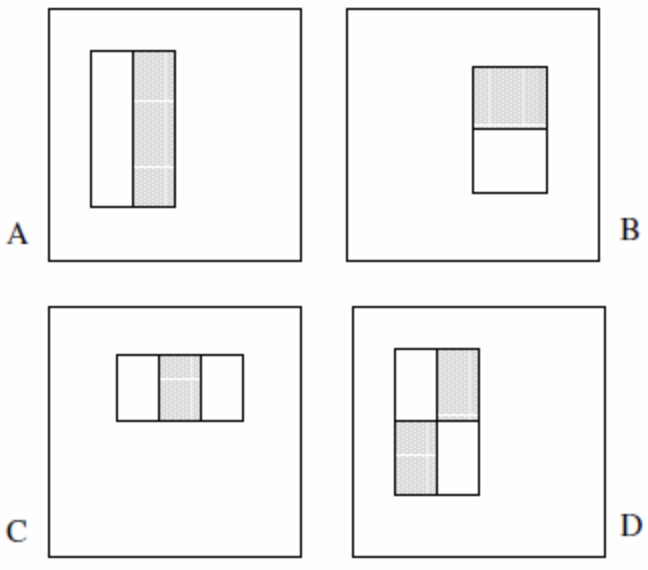
\includegraphics[width = 0.75\textwidth]{./Images/viola-jones.jpg} 
\caption{A set of Haar features used to detect faces in the Viola-Jones method. The pixels in the white regions are summed and subtracted with the pixels in the black region. The algorithm will later decide if a specific feature has been found or not, depending on obtained value.}
\end{center}
\end{figure}

This method is based on the fact that every face shares some basic similarities. Even objects of the same type can share some similarities.
\\\\
Another way to find objects in an image is to try to classify each pixel as either background or foreground, usually referred to as Foreground/Background-segmentation. This usually requires some background knowledge of how the background usually looks like, for example, if the background is grass or a concrete floor.

One of the most basic functions for separating background and foreground is the flood fill method.
Anyone that has used Paint for Windows knows exactly what this one is. It fills a segment of similar pixels with the same color. This method works best on one backgrounds with only one color.
Online there are many different variations but they all accomplish the same goal.\cite{floodFill}

One possible way of detecting objects in an image is to use depth data, or RGB-D which is depth data embedded in an RGB photo.
A popular device that uses depth data for object detection is the Kinect camera
for Xbox.

On the iPhone X, depth data can be captured by either True Depth on the front camera or with the dual cameras on the back. The True Depth camera works by having a dot projector emit light dots (mainly on a face which is why this feature is found on the front camera) and picking those dots up with an infrared camera.

The dual camera on the back works by taking two photos and comparing those to find the pixel shifts of the same objects. The distance is calculated by \[ \frac{pixelShift} { pixelFocalLength \cdot baselineInMeters}\] and gives the unit in $1/meter$. It is the same principal to how we humans see distance by having two eyes pointing the same direction. \cite{depthMap}

However, obtaining the depth data from the dual cameras in real time is not possible since it requires too much computational power. This unfortunately makes it impossible to use in an ARScene and thus not possible for this project.\\

Despite all the available methods above, object detection without machine learning is still very tricky. These methods work best when the images are in an controlled environment, typically industrial, like finding screws on a white background (as they do in an article posted by combine.se). \cite{combine}
When the environment is a more casual place though, e.g., recognizing furniture indoors, the task becomes much more difficult. For this reason, object detection with pure algorithms is not very common in household applications. Instead object detection with machine learning methods such as R-CNN's (Regional-Convolutional Neural Network) are much more common nowadays.

\section{MATLAB prototype for Object Detection}
\label{sec:ODmatlab}
% Write about design decisions for the Matlab prototype and what it does. 
% Probably add some code as well.
A purely feature based object segmentation method was implemented as a prototype in MATLAB. This was done to see if a machine learning model for detecting objects could be dismissed. 
The idea was that if one sent an image into the system, the resulting output would be bounding box coordinates for each respective object within the image. These smaller sub-images would later be separately classified using a deep neural networks. The bounding boxes would also be useful for user interface in the application. 

First, an edge detection method was run on the entire image, to find the edges, which would serve as a good variable for the segmentation. Then, Bradley's threshold algorithm \cite{Bradley} would binarize the image. Bradley's method is locally adaptive and computes the threshold value for each pixel by looking at the mean intensity of a neighborhood of pixels surrounding it.  From this, one can find enclosed blobs, and by finding enclosed blobs containing more than a certain amount of pixels, to remove noisy errors, one can find the objects. The bounding boxes are then found by selecting the minimal and maximal height and weight values of the blobs.

\section{Results from doing object detection in MATLAB}
\label{sec:ODresults}
A MATLAB script was tried in order to find possible ways of segmenting out regions containing objects in an image. The output segments would then each be classified separately. This way we would have both object locations and classifications on each object. Figure \ref{fig:matlabImages} shows an example of when this method worked. However, results from this were highly unpredictable and the parameters were too dependent on lighting, shadows, the background among other features. Figure \ref{fig:badMatlabImage} shows an example of when applying the same method on a different input image. Because of these unreliable results, this method was scrapped.


\begin{figure}[hbtp]
\begin{center}
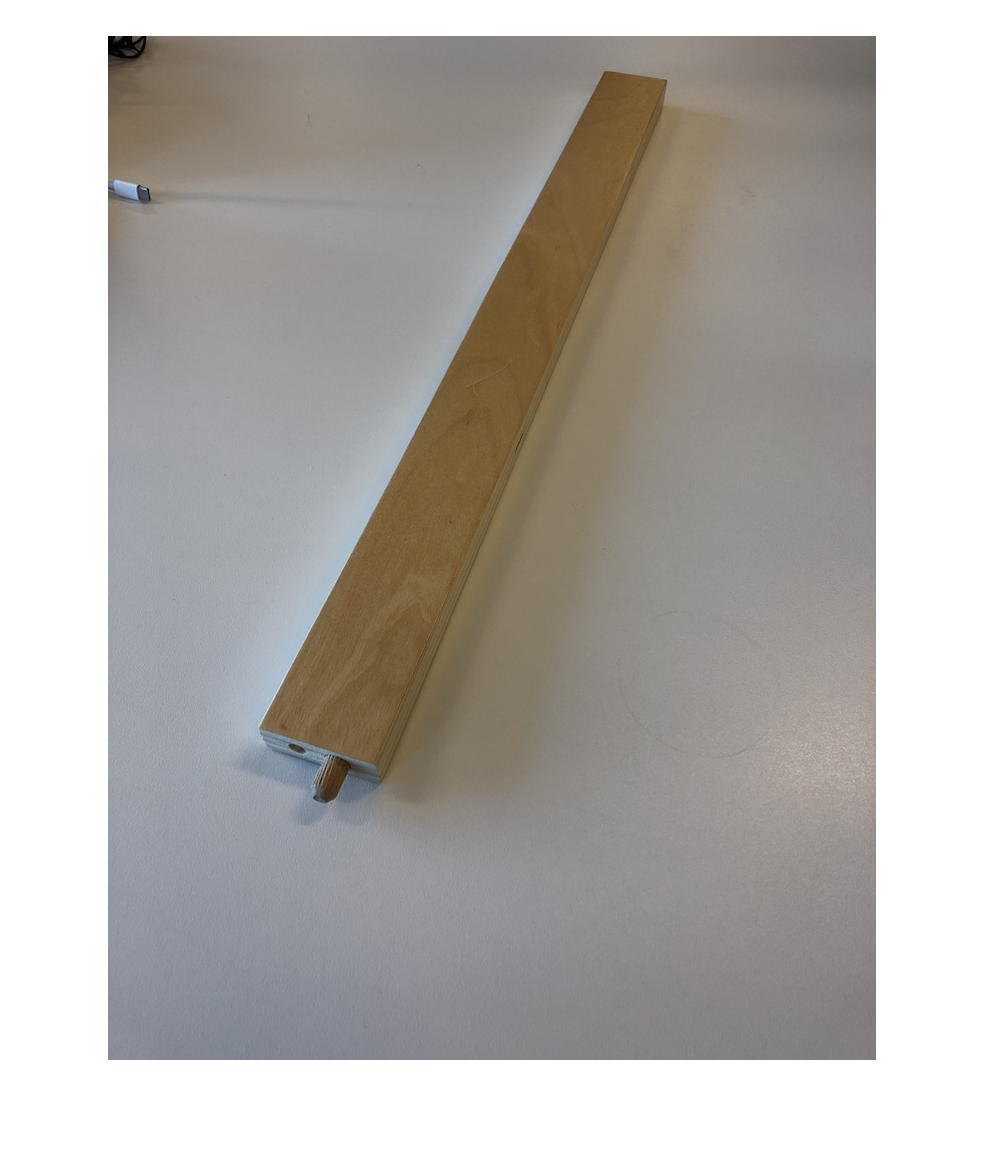
\includegraphics[width = 0.4\textwidth]{./Images/matlabImage1.png}
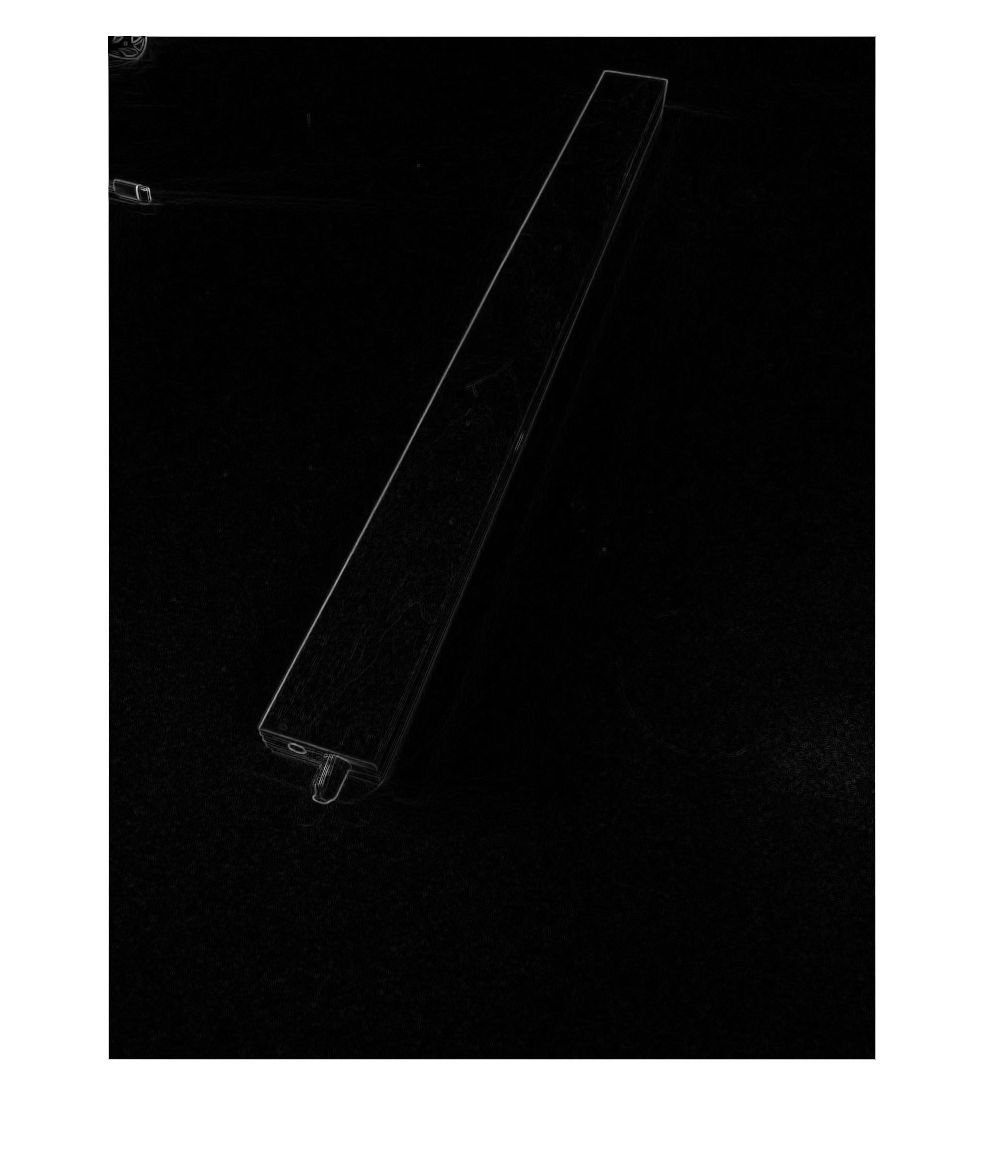
\includegraphics[width = 0.4\textwidth]{./Images/matlabImage2.png}
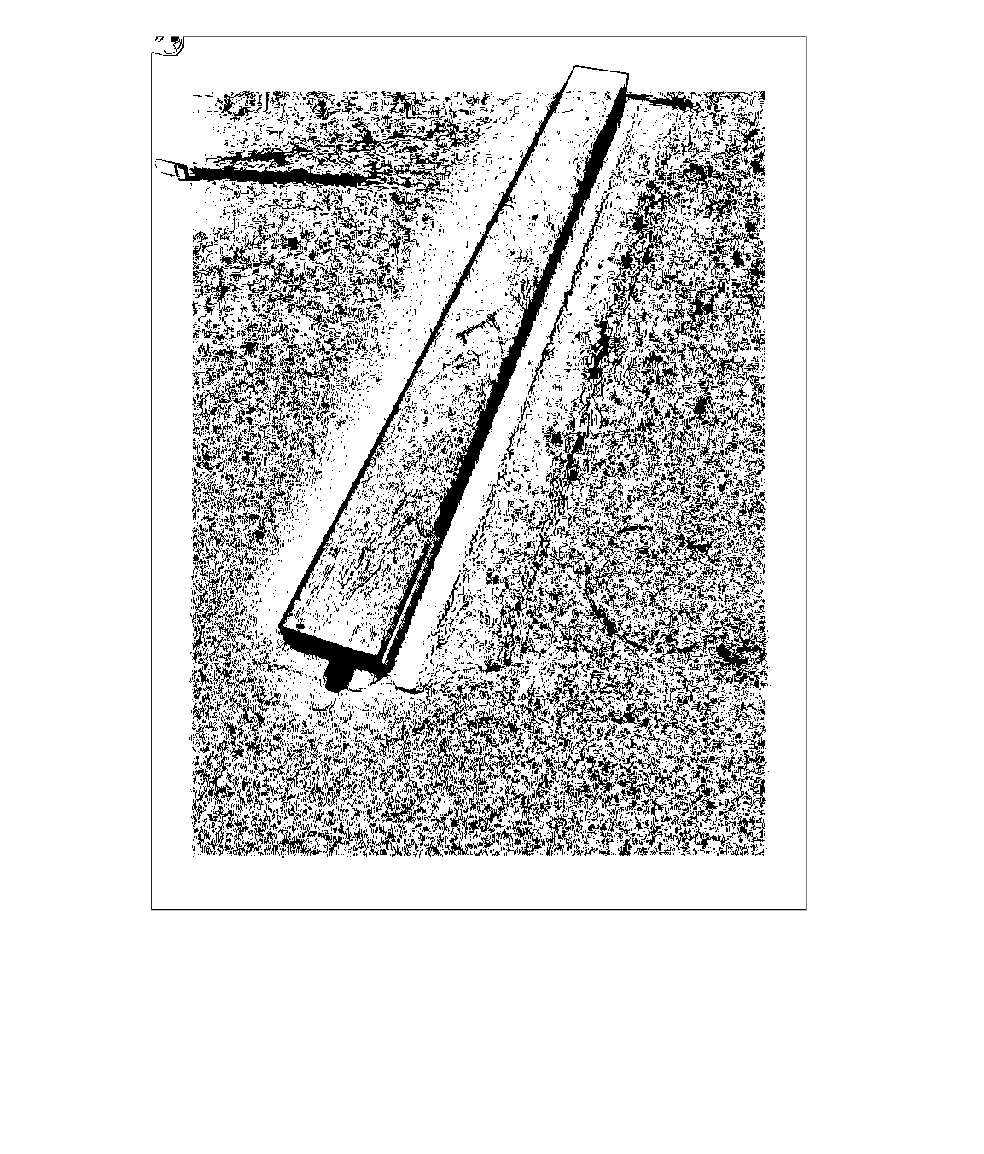
\includegraphics[width = 0.4\textwidth]{./Images/matlabImage3.png} 
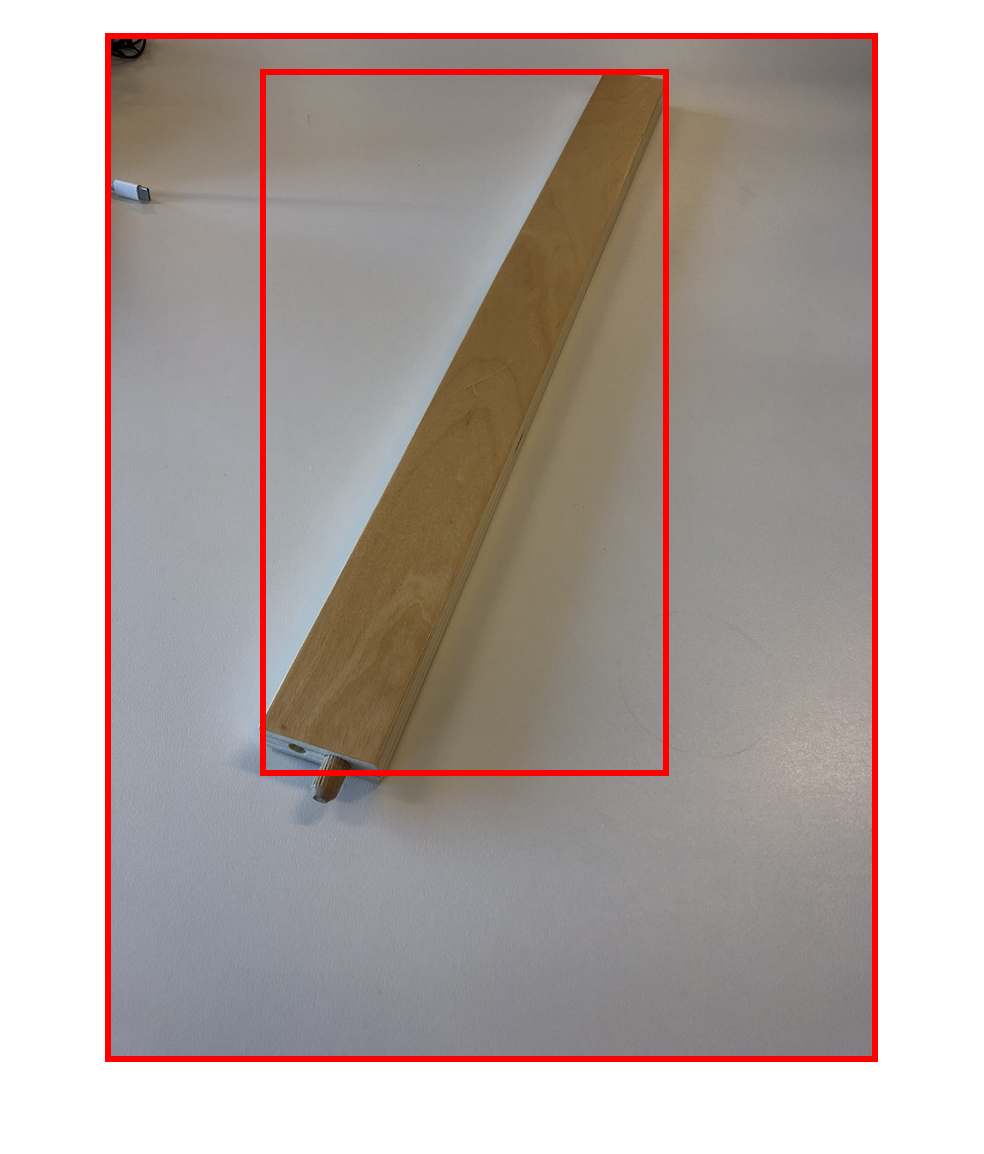
\includegraphics[width = 0.4\textwidth]{./Images/matlabImage4.png} 
\caption{Images showing the results from doing object detection in MATLAB. Top left image shows the original image. The top right image shows the result from running edge detection on the original image. Bottom left image shows the the result after binarizing the top right image. the bottom right image shows the generated bounding box superimposed on the original image}
\label{fig:matlabImages}
\end{center}
\end{figure}

\begin{figure}[hbtp]
\begin{center}
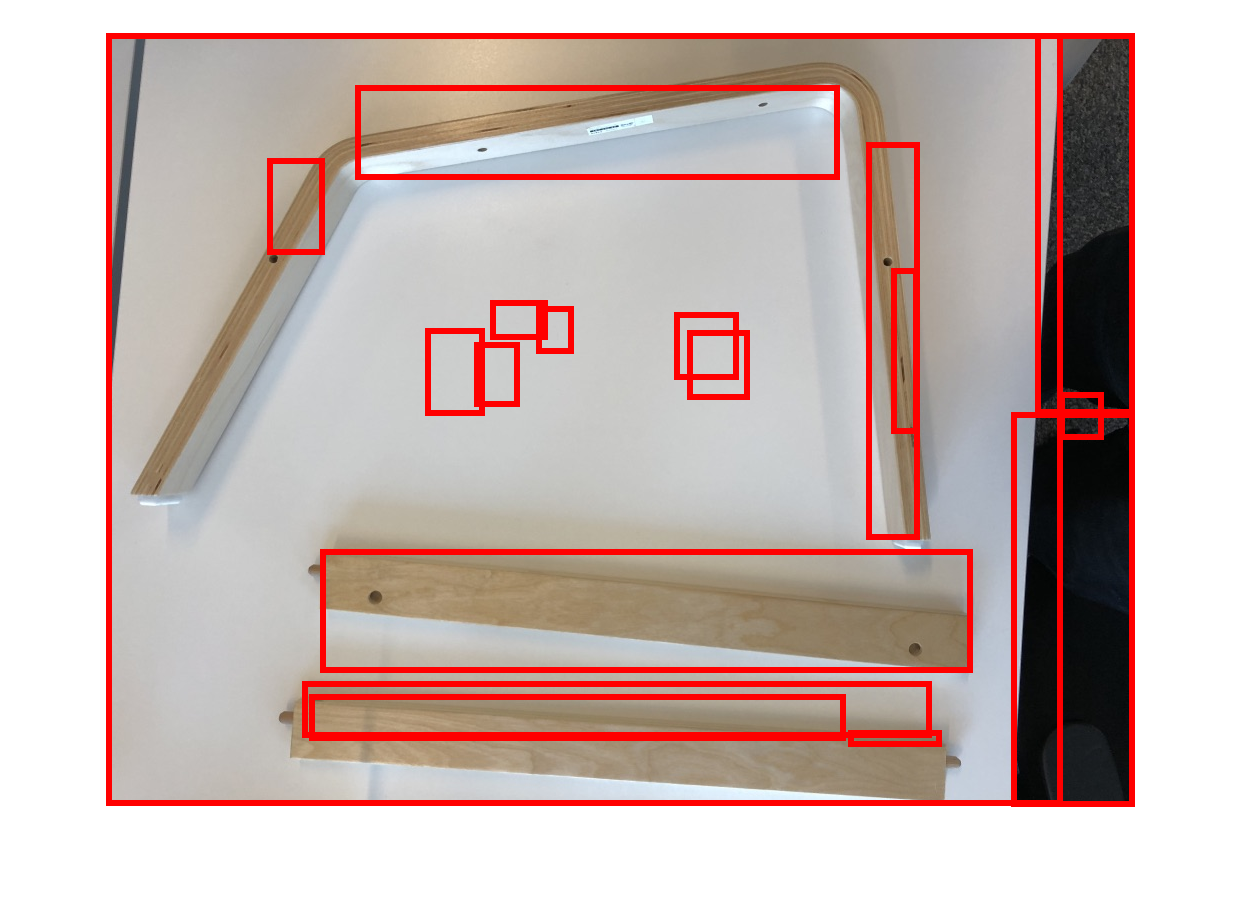
\includegraphics[width = 0.5\textwidth]{./Images/badMatlab.png}
\caption{Example image of when this method did not work as well.}
\label{fig:badMatlabImage}
\end{center}
\end{figure}

\newpage